\section{Estado del arte: bases de datos NoSQL}
\label{sec:state_dataScience}

\subsection{Introducción}
\label{subsec:state_dataScience_intro}

Un sistema gestor de bases de datos NoSQL es aquél que prescinde del modelo
relacional a la hora de almacenar la información, y por ende del SQL tradicional
como lenguaje de consultas. Éstas surgen debido a algunas carencias o problemas
de las bases de datos relacionales, principalmente la \textbf{escalabilidad
  horizontal}, es decir, la adición de nuevos nodos para reducir el
\emph{downtime} del sistema en general.

\subsection{Tipos de bases de datos NoSQL}
\label{subsec:state_NoSQL_types}


Existen varios tipos de bases de datos NoSQL, generalmente clasificadas por el
modelo de datos que emplean. Éstas clasificaciones no deberían ser tomadas
literalmente, ya que muchas de las bases de datos que mencionaremos como
ejemplos, implementan varios modelos de datos al mismo tiempo.

\paragraph{Teorema de CAP}
\mbox{}\\

En los sistemas distribuidos, el \textbf{teorema de CAP}, formulado por Eric
Brewer, dice lo siguiente:

\begin{capTheorem}
  Es imposible para un sistema distribuido ofrecer más de dos de las siguientes
  garantías al mismo tiempo: consistencia, disponibilidad y tolerancia de particiones.
\end{capTheorem}

En el contexto del teorema, cada una de las garantías se define tal que:

\begin{itemize}
\item \textbf{Consistencia: } Cada lectura recibe como respuesta la escritura
  más reciente, o un error.
\item \textbf{Disponibilidad: } Cada petición recibe una respuesta no-errónea,
  sin garantizar que contenga la escritura más reciente.
\item \textbf{Tolerancia de particiones: } El sistema continúa funcionando
  aunque se degrade el funcionamiento de la red entre los nodos, o se pierdan
  mensajes entre ellos.
\end{itemize}

En realidad, la elección real es entre o consistencia, o disponibilidad, ya que
debido al hecho de que una caída de parte del sistema no es común, únicamente
nos vemos en la situación de escoger entre consistencia o disponibilidad, cuando
ocurre un particionado en el sistema. Mientras el sistema esté funcionando con
total normalidad, se puede garantizar tanto la disponibilidad como la
consistencia del mismo.

Si el sistema permite la lectura antes de que todos los nodos tengan la última
información escrita, el sistema será catalogado como uno consistente y
tolerante a particiones (CP), mientras que si bloquea las lecturas hasta que
todos los nodos se hayan actualizado, el sistema será disponible y tolerante a
particiones (AP).

\subsubsection{Almacenes de columnas}
\label{subsubsec:state_NoSQL_types_column}

Los almacenes de columnas, bases de datos tabulares o orientados a columnas, son
bases de datos que en lugar de serializar los datos en forma de filas como lo
haría un SGBD relacional, lo hace en columnas. Veamos un ejemplo:

Gracias a éste sistema, operaciones como consultar todos los registros que contengan
un valor específico son mucho más eficientes en éste tipo de de SGBDs. Debido a
ésto, resultan ideales en entornos OLAP (\emph{Online analytical processing},
procesado analítico en línea), en los que generalmente el volumen de lecturas
es mucho mayor al de inserciones / actualizaciones.

Ejemplos: Apache Cassandra, SAP Hana, Sybase IQ

\subsubsection{Bases de datos documental}
\label{subsubsec:state_NoSQL_types_doc}

En una base de datos documental, la información se almacena en un formato
semi-estructurado: es decir, con ficheros siguiendo un formato de documento
específico, como podrían ser XML, JSON y YAML.

Éstos tipos de documentos almacenan toda la información referente al objeto que
describen en el mismo documento, permitiendo que se añada información a
documentos específicos sin tener que mantener una estructura consistente en
todos los documentos.

En el espectro del teorema CAP, las bases de datos documentales se sitúan principalmente en
el vértice de la tolerancia de particiones. Las bases de datos documentales AP (Available,
partition-tolerant) como 

\subsubsection{Almacenes clave-valor}
\label{subsubsec:state_NoSQL_types_keyval}

Las bases de datos clave-valor almacenan la información en \emph{arrays}
asociativos, o dicho de otra manera, diccionarios. Cada diccionario contiene
registros o objetos, y de la misma manera que en las bases de datos
documentales, cada uno puede albergar diferente información.

En éstas bases de datos, el valor de una clave es completamente opaco, por lo
que es imposible filtrar por el contenido del registro. Al no disponer de
lenguaje de consultas, la interacción con la base de datos se realiza mediante
los comandos \texttt{get}, \texttt{put} y \texttt{delete}.

\subsubsection{Bases de datos orientada a grafos}
\label{subsubsec:state_NoSQL_types_graph}

Los grafos son una estructura de datos, que modelan la información según
relaciones entre objetos:

\begin{figure}[ht!]
  \centering
  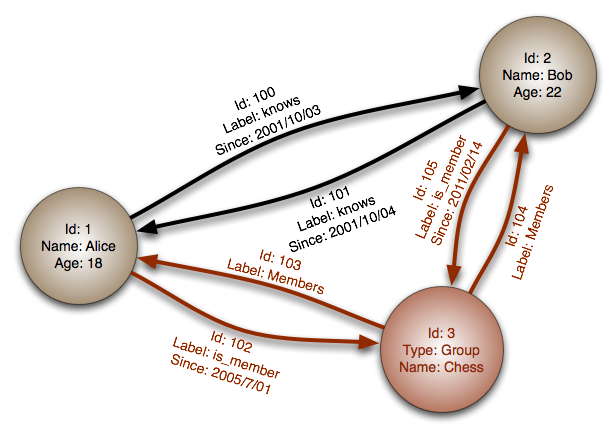
\includegraphics[scale=0.75]{img/graphDB.png}
  \caption{\label{fig:grafo} Base de datos de grafos}
\end{figure}
\
Los grafos se basan en los siguientes tres conceptos:

\begin{enumerate}
\item Los \textbf{nodos} representan cualquier entidad, y se pueden considerar
  equivalentes a otros objetos como un registro en una base de datos relacional,
  documento en una documental, y así.
 \item Las \textbf{aristas}, también llamadas relaciones, son las líneas que
   conectan los nodos, representando las relaciones entre ellos.
 \item Las \textbf{propiedades} son etiquetas asociadas a los nodos
   nodo.
\end{enumerate}

En contraste a las bases de datos relacionales, éstas almacenan directamente las
relaciones entre nodos, por lo que, en teoría, las consultas que deban enlazar información
son más veloces en bases de datos de grafos, ya que un SGBD relacional debe
realizar una \emph{join} en dos tablas diferentes. Ésta eficiencia se va
acentuando conforme la complejidad de la consulta aumenta: una base de datos
orientada a grafos sólo debe seguir las aristas a partir del nodo inicial.

Algunos ejemplos de bases de datos orientadas a grafos son AllegroGraph, Neo4j y
Openlink Virtuoso.

\subsubsection{Bases de datos orientadas a objetos}
\label{subsubsec:state_NoSQL_types_object}

En éste tipo de bases de datos, la información se almacena como objetos en el
paradigma homónimo. Según el ``Object-Oriented Database Manifesto'', las bases
de datos orientadas a objetos difieren de la serialización de los mismos en que
deben proveer concurrencia, capacidad de recuperación, y algún mecanismo para
consultar sobre éstos objetos.